\chapter{Framework Modules}
\section{Module: Core-Framework}
\label{sec:core}
\subsection{Network}
The network implementation has the concept of leechers and seeders. A leecher connects to one or more seeders and requests chunks from them. A seeder has multiple leechers connected to it and answers to chunk requests. Every chunk transfer is pull-based, which means it can only be requested by the leecher while every non-chunk transfer like Meta-Data or address announcements is always push-based, which means that a seeder transfers them without being asked to do so. This has the advantage that every leecher knows exactly what a seeder has to offer without asking but only requests the chunks it needs. See section \ref{subsubsec:downloadreq} for more information.

While leechers and seeders are independent of each other it is possible to couple them together. A leecher coupled with a seeder always announces the address of its seeder to any other seeder it is connected with. This concept is explained in more detail in section \ref{subsubsec:autoconnect}.

Both a leecher and a seeder keep a reference to a database instance. A leecher stores downloaded chunks in its database and a seeder uploads chunks from its database. It is possible that both a leecher and a seeder reference the same database instance in which case the seeder is able to upload every downloaded chunk from the leecher. The DataBase module and all related concepts are explained in section \ref{sec:database}.

A leecher and a seeder both are associated with one of the multiple distribution algorithms defined in the Algorithm module. Those algorithms determine the distribution behaviour, which is further described in section \ref{sec:algorithm}.

\subsubsection{Automatic Connect}
\label{subsubsec:autoconnect}
While every leecher has to manually connect to a seeder for the first time, after this a leecher is able to automatically connect to other seeders. This is because every leecher who is coupled with a seeder announces the address of its coupled seeder to all other seeders it is currently connected with. The figure \ref{fig:autoconnect} show this in detail.

\begin{figure}[H]
\centering
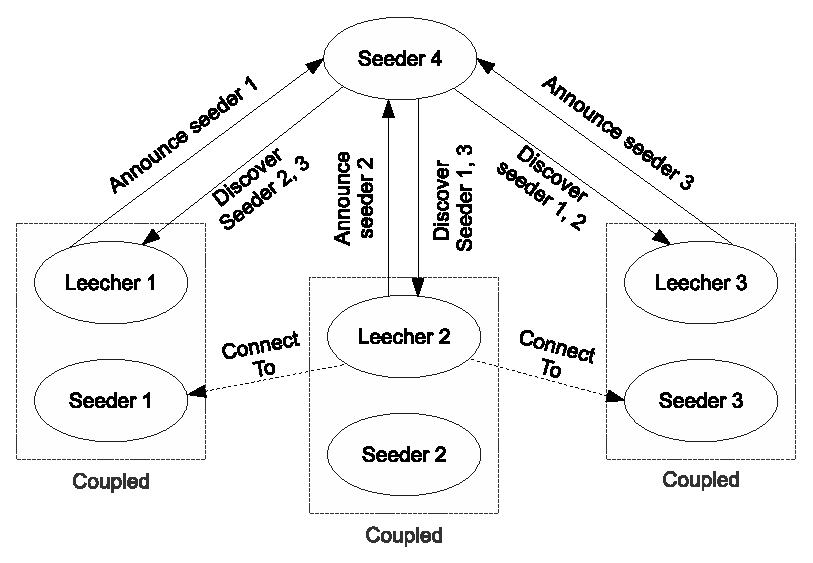
\includegraphics[width=8cm]{autoconnect}
\caption{Seeder Discovery}
\label{fig:autoconnect}
\end{figure}

Here leecher 1, 2 and 3 announce the address of seeder 1, 2 and 3 respectively to seeder 4 which then broadcasts those addresses to all connected leechers. This way the leechers get to know each other and can connect to the remaining seeders. Though in figure \ref{fig:autoconnect} only leecher 2 is illustrated, leecher 1 and 3 connect to the other seeders as well. Of course, this works recursively, so if one of the seeders 1, 2 or 3 already has other leechers connected to it those will also be found. So in the end the topology is just a mesh with $(n-1)*n$ connections where $n$ refers to the total number of coupled seeders and leechers and every leecher of each couple is connected to every seeder of all other couples. The figure \ref{fig:mesh} shows a mesh of 4 couples where every line counts for two connections.

\begin{figure}[H]
\centering
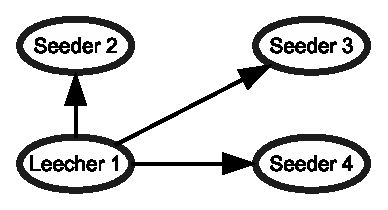
\includegraphics[width=8cm]{mesh}
\caption{Mesh topology}
\label{fig:mesh}
\end{figure}

While this topology is really great in terms of knowledge where every peer knows exactly what data sets the other peers have and thus can request chunks efficiently, it is also quite expensive and would not scale indefinitely. To improve scalability and reduce efficiency the number of connections per leecher can be limited which limits the knowledge of each leecher and thus the ability to make good decisions what to request from whom. This is explained later in section \ref{sec:benchmark} in more detail.

If a leecher loses, for what ever reason, the connection to a seeder the framework is able to reconnect if the seeder is still online. This will be detected by periodic address broadcasts. So if, for instance, leecher 1 lost the connection to seeder 2 but leecher 1 and 2 are also connected to seeder 3 then seeder 3 will notify leecher 1 that seeder 2 still exists. The figure \ref{fig:reconnect} illustrates this.

\begin{figure}[H]
\centering
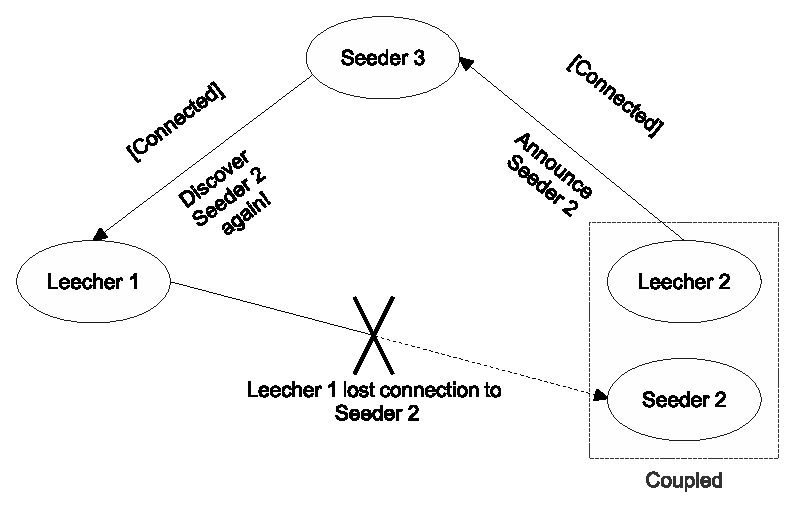
\includegraphics[width=8cm]{reconnect}
\caption{Reconnect}
\label{fig:reconnect}
\end{figure}


\subsubsection{Meta-Data Announcements}
After a leecher connects to a seeder the leecher does not know anything about the seeder. As previously explained in section \ref{subsubsec:autoconnect} the leecher discovers new seeders through the seeders it is currently connected to. The way the leecher gets knowlege about what data sets a seeder offers works a similiar way. A seeder announces to all connected leechers periodically what data sets it has to offer. It basically transfers a list of Meta-Data, which is explained further in section \ref{subsubsec:metadata}, so that every leecher can update its knowledge about the seeder. The list of Meta-Data can be modified before it is announced by the used distribution algorithm to model a specific distribution behaviour, see section \ref{sec:algorithm} for further information.

As an optimization the seeder only transfers new Meta-Data. So if a data set does not change at all, a seeder will never transfer a second announcement of this data set. Another optimization is that while a leecher downloads a chunk from a seeder, the seeder will also not transfer any announcements during this period, which is explained further in the next section \ref{subsubsec:downloadreq}.


\subsubsection{Download Requests}
\label{subsubsec:downloadreq}
After a leecher successfully connected to one or more seeders and already received Meta-Data announcements it can start to request chunks from the seeders. What to request from whom heavily depends on the used distribution algorithm, which is explained in section \ref{sec:algorithm} in more detail. 

Since downloading more than one chunk at a time from a seeder is not faster than downloading them sequentially only one download at a time is allowed which also reduces protocol complexity. Because of that Meta-Data and address announcements are also not transferred during a chunk download because those announcements are then obviously of no interest for the leecher. As soon as the chunk download completes outstanding announcements are bundled and transferred.

A seeder is allowed to decide whether or not a chunk request is valid, which means that depending on the algorithm the seeder can reject a chunk request. If a seeder rejects a chunk request the leecher do not request the same chunk again. The seeder can tell the leecher that a previously rejected chunk request is valid again by reannouncing the specific chunk. This way complex distribution behaviour can easily be implemented.


\subsubsection{Nonblocking I/O}
Network communication is based on sockets. Sockets can either be datagram or stream based. Datagram sockets have no notion of connections and are of no importance for this thesis. Instead the network implementation uses stream sockets. A stream socket is always connected to an other socket. Those two sockets behave like files. If you write data to a socket it is transferred to the other socket and can then be read from it. As with files, socket operations usually block the currently executing thread until the requested data is read or written. This implies that you basically need one thread per socket to handle multiple sockets concurrently. Unfortunately threads are a limited resource and thus this concept does not scale well. 

To improve this situation nonblocking sockets in combination with event-polling were introduced, where you are notified when a socket operation can be executed without blocking. This way you can theoretically serve tens of thousands of sockets in a single thread. Since this thesis concentrates on large-scale this technique is a must-have.

The problem with nonblocking sockets is that it increases the complexity significantly so the network implementation uses a framework to simplify the usage. The framework is called Netty 5 and written in Java. One great thing about Netty is that it totally separates the transport protocol oriented code from the logic oriented one. This way it does not matter which transport protocol you use as long as this protocol is stream based.


\subsubsection{Transport: Local and TCP}
Netty offers a Local (also called In-VM) transport protocol which does not involve network at all. It only works inside a single instance of the JVM and is perfectly suited for simulations or benchmarking. That is because the Local transport does not require you to serialize and deserialize the data which eliminates a huge amount of memory and CPU usage. In normal usage the overhead of serialization is negligible but since the Benchmark module is able to simulate a large number of seeders and leechers, see section \ref{sec:benchmark}, those overheads can start to sum up. The Local transport seems to be the perfect fit for this purpose.

Netty also offers usual transport protocols like TCP. It is used as secondary option for the Benchmark module which is useful if you want to run distributed benchmark on multiple machines since Local transport is limited to a single JVM instance.


\subsubsection{Traffic-Shaping}
To simulate and evaluate network applications you need the ability to control the bandwidth in some way to have comparable network conditions. The problem with bandwidth limitation, which is also called traffic-shaping, is that most times you cannot throttle the writer. The writer can either be writing as fast as possible or not writing at all. So in order to limit the bandwidth you have to start and stop the writer periodically. Because readers and writers are identical in terms of bandwidth limitation the explanation always refers to writers but the same approach works for readers equally well .

If the period is too long the introduced bandwidth peaks can affect the measurements in a negative way but if the period is too short instead, you introduce a lot of overhead. To perfectly limit the bandwidth you would need to use a period which is indefinitely short. So if you want to implement traffic-shaping reliably, you must find the sweet spot between accuracy and minimal overhead. The network implementation uses a period of 250 ms which is good enough because the measurements are done every second. So every measurement contains the average of approximately 4 bandwidth limitation runs.

The complexity increases if multiple writers together are not allowed to exceed a given bandwidth. The main problem is fairness. You do not want that one writer gets 95\% of the bandwidth while the remaining writes get only 5\% together. But at the same time you want that a single writer is able to write at full speed if no other writer is writing. This complex behaviour can be achieved using a Leaky-Bucket algorithm and a Priority-Queue.

The Leaky-Bucket contains tokens, where one token equals one byte. If a writer wants to write a message it tries to remove the tokens needed for the message to transfer. If the bucket does not have enough tokens, the writer takes the remaining tokens and decreases the size of the message it want to write by the number of removed tokens. After this it waits until the bucket gets refilled and repeats the action. Unfortunately this does not fix the fairness problem.

To solve the fairness problem a writer is not allowed to remove tokens from the bucket directly. Instead it inserts the write request into a Priority-Queue. A writer-job constantly polls the head of the queue and tries to process the write request using the Leaky-Bucket. The difference is that after writing the message the writer increases its number of total written bytes. If the writer has more messages to write it inserts itself into the queue according to the number of total written bytes compared to other writers. This way the head of the queue always is a write request belonging to a writer which has written least. This way you get good fairness with almost no overhead because the writer-job runs only on demand in a thread pool and quits after all write requests are processed.

\cleardoublepage
\subsection{Concurrency}
With the use of nonblocking sockets it is possible to handle a lot of sockets with only one thread. But this can be further improved because modern CPUs always have multiple cores whose quantity determines the number of threads able to run in parallel. If your CPU has 4 cores and you are using only one thread then you cannot use more than 25\% of your CPU capacity. Because of that Netty uses more than one thread to increase the efficiency. In the next section \ref{subsecsec:eventloop} the utilization of multiple threads is explained in more detail.

\subsubsection{Event-Loop}
\label{subsecsec:eventloop}
Netty has the notion of an Event-Loop. An Event-Loop is always running in its own thread and processes queued events one after the other. Those events are mostly readiness events which say that a given socket is now readable, writable, acceptable or connectable.

To use more than one thread Netty simply spawns more Event-Loops, typically just as many as there are CPU cores. New sockets will then be distributed evenly among all running Event-Loops. Even if the Event-Loops get unbalanced Netty tries to rearrange the sockets to become balanced again.

Those Event-Loops can then run theoretically in parallel, because the underlying operating system distributes busy threads equally among all available cores. But using more than one thread is only the tip of the iceberg, multiple threads introduce a whole new category of problems and considerations which have to be taken into account. The next section \ref{subsecsec:lockfree} discusses this a bit more in depth.


\subsubsection{Lock-Free-Progamming}
\label{subsecsec:lockfree}
The main problem when using multiple threads is the question of how those threads interact which each other. If two threads access the same variable without any protection the resulting behaviour is not always defined and can lead to untraceable bugs. The unprotected access of variables is called a critical-section.

A simple solution is to protect those sections with a mutually exclusive (mutex) lock, which simply forbids that more than one thread is entering the critical-section at a time, but this decreases efficiency and increase thread context switching, which is expensive. One solution is to use lock-free algorithms, which exploit certain guarantees made by the Java Memory-Model. To explain those concepts in detail would arguably exceed the boundries of this thesis, but it should be noted that the network implemention heavily uses those algorithms.

The reason why those concepts were considered is that inter-thread-communication was a key design choice in order to simplify the architecture of the implementation. For instance a leecher can be connected to a lot of seeders receiving a lot of Meta-Data and address announcements. In order to effectively request chunks from the seeders the leecher has to collect the information from all connections which may run in different threads and thus are not protected against concurrent access by default. Since this collection is a very common task it should be optimized as well. Using CAS and volatile operations the necessary mutexes can be reduced to a minimum. 

In normal situations the overhead of mutexes can be ignored, but when simulating hundreds of leechers and seeders on multiple cores this means a lot of cross thread access. If every collection of Meta-Data of each leecher would stop all Event-Loop threads by using a mutex the overhead should start to be noticeable. Those impacts are hard to measure or quantify, though. But in principle the lock-free approach scales better. As a rule of thumb lock-free-algorithms should always be preferred in performance critical sections.

\cleardoublepage
\section{Module: DataBase}
\label{sec:database}
The DataBase module represents a generic interface for storing binary data in any kind of storage. While the Core-Framework transfers data between peers the data has to be read from and written to some kind of database. The data managed by the database is not just plain data but chunked data instead. Because of that a database stores so called data sets which consist of multiple chunks. 

The database has the responsibility to verify stored chunks in terms of consistency and validation. But to do so the storage has to know about the structure of the data set. Because of that the Meta-Data which describes a given data set is stored together with the data set as key-value pairs. The next section \ref{subsubsec:metadata} describes the Meta-Data format in more detail.

\subsubsection{Meta-Data}
\label{subsubsec:metadata}
The Meta-Data contains information about a given data set. Those information are transferred between seeders and leechers to describe what data sets are avaiable for download. Those information are:
\begin{itemize} 
\setlength{\parskip}{1pt}
\item Name
\item Description
\item ID
\item Size
\item Chunks
\item Hash
\item ChunkHashes
\end{itemize}
The Name and Description fields are used for human-related tasks. The ID has to be globally unique and is used for streaming purposes which will be explained later in section \ref{sec:streaming}. The Size field determines the total size of the data set including all chunks which leads to the next field. The Chunks field is a bit set which simply stores one or zero bits for existing or missing chunks respectively. The length of the bit set determines the number of chunks a data set has. The Hash field contains a checksum generated by a strong hash algorithm like SHA from the whole data set. The ChunkHashes field does the same but for each chunk individually. This way the storage can verify single chunks as well as the data set in total. The reason why there is an extra Hash field for the whole data set is to reduce the chance of hash collision. Two data sets are equal if all of their fields are also equal.

\subsubsection{Backends: In-Memory and Filesystem}
The In-Memory backend stores data sets in main memory and is not persistent. It is a useful backend for situations where you generate or consume data sets on the fly like video streaming or test scenarios.

In case of streaming you could simply add fake data set sources which loads chunks from a live camera or similiar devices.

The Benchmark module uses this backend to reduce overhead introduced by the filesystem. This backend almost has no overhead other than memory usage.

Related to future work is the filesystem backend which implements a persistent database based on a filesystem. The filesystem can also be virtual like a ZIP file. This backend is more rigid but also very important for file-sharing applications.

\cleardoublepage
\section{Module: Algorithm}
\label{sec:algorithm}
This module contains the logic of the whole implementation. While the Core-Framework module takes care of all the low-level parts the real work is done here. This module defines two interfaces for both a seeder and a leecher which are called SeederDistributionAlgorithm and LeecherDistributionAlgorithm respectively. 

A SeederDistributionAlgorithm can modify Meta-Data which is announced by a seeder and allows or rejects chunk requests. A LeecherDistributionAlgorithm is even simpler, it can only request chunks. A simplified implementation of both interfaces would look like this:

\begin{verbatim}
interface SeederDistributionAlgorithm {
    list of metaData modifyMetaData(list of metaData);
    boolean isChunkRequestAllowed(chunkRequest);
}

interface LeecherDistributionAlgorithm {
    list of chunkRequest requestChunks(availableDataSetsOfAllSeeders);
}
\end{verbatim}

As you can see, those interfaces are totally independend of the underlying network implementation. The core concept is that a leecher algorithm is only interested in requesting chunks as efficient as possible. The seeder can decide if a requested chunk request is allowed or not and what Meta-Data it announces. With those two methods a seeder can model the behaviour of a seeder which uploads to everybody, or only one upload in total, or even stop announcing Meta-Data if the associated data sets have already been transferred, which is used by the SuperSeederChunkedSwarm algorithm, which is explained in section \ref{subsubsec:superseederchunkedswarm}.

\subsubsection{Algorithm: Sequential}
\label{subsubsec:sequential}

\subsubsection{Algorithm: Logarithmic}
\label{subsubsec:logarithmic}

\subsubsection{Algorithm: ChunkedSwarm}
\label{subsubsec:chunkedswarm}

\subsubsection{Algorithm: SuperSeederChunkedSwarm}
\label{subsubsec:superseederchunkedswarm}

\cleardoublepage
\section{Module: Monitoring}
\label{sec:monitoring}

